%%%%%%%%%%%%%%%%%%%%%%%%%%%%%%%%%%%%%%%%%
% Masters/Doctoral Thesis 
% LaTeX Template
% Version 1.43 (17/5/14)
%
% This template has been downloaded from:
% http://www.LaTeXTemplates.com
%
% Original authors:
% Steven Gunn 
% http://users.ecs.soton.ac.uk/srg/softwaretools/document/templates/
% and
% Sunil Patel
% http://www.sunilpatel.co.uk/thesis-template/
%
% License:
% CC BY-NC-SA 3.0 (http://creativecommons.org/licenses/by-nc-sa/3.0/)
%
% Note:
% Make sure to edit document variables in the Thesis.cls file
%
%%%%%%%%%%%%%%%%%%%%%%%%%%%%%%%%%%%%%%%%%

%----------------------------------------------------------------------------------------
%	PACKAGES AND OTHER DOCUMENT CONFIGURATIONS
%----------------------------------------------------------------------------------------

\documentclass[11pt, oneside]{Thesis} % The default font size and one-sided printing (no margin offsets)

\graphicspath{{Pictures/}} % Specifies the directory where pictures are stored

\usepackage[figurewithin=none,tablewithin=none]{caption}
\usepackage[round, comma, sort&compress]{natbib} % Use the natbib reference package - read up on this to edit the reference style; if you want text (e.g. Smith et al., 2012) for the in-text references (instead of numbers), remove 'numbers' 
\hypersetup{urlcolor=blue, colorlinks=true} % Colors hyperlinks in blue - change to black if annoying
\title{\ttitle} % Defines the thesis title - don't touch this

%\renewcommand{\thetable}{\arabic{table}}
%\renewcommand{\thefigure}{\arabic{figure}}

\begin{document}

\frontmatter % Use roman page numbering style (i, ii, iii, iv...) for the pre-content pages

\setstretch{1.3} % Line spacing of 1.3

\pagestyle{fancy}
\fancyhf{}
\rhead{\thepage}
\lhead{\thechapter}
\cfoot{\thepage}

% Define the page headers using the FancyHdr package and set up for one-sided printing
%\fancyhead{} % Clears all page headers and footers
%\rhead{\thepage} % Sets the right side header to show the page number
%\lhead{} % Clears the left side page header
%\pagestyle{fancy} % Finally, use the "fancy" page style to implement the FancyHdr headers

\newcommand{\HRule}{\rule{\linewidth}{0.5mm}} % New command to make the lines in the title page
\renewcommand{\bibname}{References}

% PDF meta-data
\hypersetup{pdftitle={\ttitle}}
\hypersetup{pdfsubject=\subjectname}
\hypersetup{pdfauthor=\authornames}
\hypersetup{pdfkeywords=\keywordnames}

%----------------------------------------------------------------------------------------
%	TITLE PAGE
%----------------------------------------------------------------------------------------

\begin{titlepage}
\begin{center}

\textsc{\LARGE Universität Potsdam}\\[1.5cm]
\textsc{\LARGE Institut für Erd- und Umweltwissenschaften}\\[1.5cm]
%\textsc{\LARGE \univname}\\[1.5cm] % University name
%\textsc{\Large Doctoral Thesis}\\[0.5cm] % Thesis type

\HRule \\[0.4cm] % Horizontal line
{\huge \bfseries Einführung in Bayessche Netze für Geowissenschaftler}\\[0.4cm] % Thesis title
\HRule \\[1.5cm] % Horizontal line
 
\emph{Author:}\\
{\authornames}

\emph{Matrikelnr.:}\\
{743289}

\emph{Email:}\\
{silvio.schwarz@uni-potsdam.de}


 

{\large June 2015}\\[4cm] % Date
%\includegraphics{Logo} % University/department logo - uncomment to place it
 
\vfill
\end{center}

\end{titlepage}


%----------------------------------------------------------------------------------------
%	LIST OF CONTENTS/FIGURES/TABLES PAGES
%----------------------------------------------------------------------------------------

\pagestyle{fancy} % The page style headers have been "empty" all this time, now use the "fancy" headers as defined before to bring them back

\lhead{\emph{Contents}} % Set the left side page header to "Contents"
\tableofcontents % Write out the Table of Contents

\lhead{\emph{List of Figures}} % Set the left side page header to "List of Figures"
\listoffigures % Write out the List of Figures

\lhead{\emph{List of Tables}} % Set the left side page header to "List of Tables"
\listoftables % Write out the List of Tables

%----------------------------------------------------------------------------------------
%	ABBREVIATIONS
%----------------------------------------------------------------------------------------

%\clearpage % Start a new page

%\setstretch{1.5} % Set the line spacing to 1.5, this makes the following tables easier to read

%\lhead{\emph{Abbreviations}} % Set the left side page header to "Abbreviations"
%\listofsymbols{ll} % Include a list of Abbreviations (a table of two columns)
%{
%\textbf{DAG} & \textbf{D}irected \textbf{A}cyclic \textbf{G}raph \\
%\textbf{PGA} & \textbf{P}eak \textbf{G}round \textbf{A}cceleration \\
%\textbf{PSA} & \textbf{P}seudo \textbf{S}pectral \textbf{A}cceleration \\
%\textbf{Acronym} & \textbf{W}hat (it) \textbf{S}tands \textbf{F}or \\
%}

%----------------------------------------------------------------------------------------
%	SYMBOLS
%----------------------------------------------------------------------------------------

%\clearpage % Start a new page

%\lhead{\emph{Symbols}} % Set the left side page header to "Symbols"

%\listofnomenclature{lll} % Include a list of Symbols (a three column table)
%{
%$a$ & distance & m \\
%$P$ & power & W (Js$^{-1}$) \\
% Symbol & Name & Unit \\

%& & \\ % Gap to separate the Roman symbols from the Greek

%$\omega$ & angular frequency & rads$^{-1}$ \\
%% Symbol & Name & Unit \\
%}

%----------------------------------------------------------------------------------------
%	THESIS CONTENT - CHAPTERS
%----------------------------------------------------------------------------------------

\mainmatter % Begin numeric (1,2,3...) page numbering

\pagestyle{fancy} % Return the page headers back to the "fancy" style

% Include the chapters of the thesis as separate files from the Chapters folder
% Uncomment the lines as you write the chapters

% Chapter 1

\chapter{Introduction} % Main chapter title

\label{Chapter1} % For referencing the chapter elsewhere, use \ref{Chapter1} 

\lhead{Chapter 1. \emph{Introduction}} % This is for the header on each page - perhaps a shortened title
The following assignment is an exam for the master course "MGEW23: Einführung in Bayessche Netze für Geowissenschaftler" in the scope of the master program "Geowissenschaften" at Universität Potsdam.\\
The purpose of this work is to use Bayesian Networks in an example that resembles simplified questions one would encounter in the assessment of natural hazards. The task is to build ground motion models from synthetic data and quantify their ability to predict values of peak ground acceleration (PGA) given the input variables.\\
In the context of this paper four Bayesian Networks have been learned. These include a causal network, a naive Bayes network, a constraint-based network using a grow-shrink algorithm and a score-based one from a hill-climber. Special care is given to the evaluation of the prediction performance. A mean squared error and a log-likelihood score are computed on a testing set in order to get an estimate of the out-of-sample performance. In a next step the concept of testing on unseen data is expanded to crossvalidation and finally an attempt of a bias-variance-decomposition is made to further develop this concept and to draw conclusion where potential for improvement lies.\\
The computations were performed using R \citep{R} in combination with the IDE RStudio \citep{Rstudio}. For setting up and working with Bayesian Networks the R package bnlearn \citep{bnlearn} was used.
% Chapter 2

\chapter{Learning Bayesian Networks} % Main chapter title

\label{Chapter2} % For referencing the chapter elsewhere, use \ref{Chapter1} 

\lhead{Chapter 2. \emph{Learning}} % This is for the header on each page - perhaps a shortened title
Bayesian networks are directed acyclic graphs (DAG). They are representations of the dependence structure among a set of random variables. The conditional dependencies between the random variables are visualized by directed edges and the random variables themselves are the nodes of the network. Through the directed edges it is possibly to identify a hierarchy. Nodes having edges leading to another node are called parents of the receiving node. Similarly, the receiving node is a child of the source node. Besides the dependence structure the nodes in a Bayesian Network carry a probability distribution conditional on their parents. In the case of discrete distributions this becomes a probability table.\\
The advantage of using a Bayesian Network is that it represents the joint probability over all the random variables considered, so that it is possible to answer conditional queries through the laws of probability theory. Through the structure of the network the joint probability distribution factorizes, leading to less parameters to estimate and a more efficient computation.\\
For the task of the evaluation of natural hazard Bayesian Networks provide a consistent and efficient way to compute the full distribution of the target variable and thus to deal with the associated uncertainties.
\newpage

%----------------------------------------------------------------------------------------

\section{Building Bayesian Networks}
The task for this assignment is to build different Bayesian Networks, use synthetic data to learn the corresponding parameters and, to evaluate their performance of predicting on the target value.\\
The data consists of a set of six variables commonly employed for defining ground motion models and the prediction of ground motion values such as PGA, PSA or macroseismic intensity. Each of the variables has been sampled from a distribution according to Table~\ref{tab:1} and the stochastic model of     \cite{boore2003} was used to compute the corresponding values of PGA. These are included in the data as log(PGA) since its values span several orders of magnitude and it is assumed that PGA follows a log-normal distribution, hence the logarithm of it is a gaussian distribution. In total the dataset comprises 10000 "observations".
\vspace{1.5cm}


\begin{table}[h]
\begin{tabular}{ p{3cm}p{5cm}p{5cm}  }
\hline
 $X_i$ & Description & Distribution$_{[range]}$\\
 \hline 
 \hline
 \multicolumn{3}{c}{Variables} \\
 \hline
 M   & Moment Magnitude    &$\mathcal{U}_{[5,7.5]}$\\
 R&   Distance to Source  & Exp$_{[1 km, 200km]}$\\
 SD & Stress drop & Exp$_{[0 bar, 500bar]}$\\
 $Q_0$    &Attenuation of seismic waves in deep strata &  Exp$_{[0 s^{-1}, 5000 s^{-1}]}$\\
 $\kappa_0$&   Attenuation of seismic waves close to the surface  &  Exp$_{[0 s, 0.1 s]}$\\
 $V_s30$& Average shear wave velocity in the upper 30m  & $\mathcal{U}_{[600 m s^{-1}, 2800 m s^{-1}]}$\\
 \hline
 \multicolumn{3}{c}{Ground Motion Variable} \\
 \hline
 $\log PGA$& logarithm of peak horizontal ground acceleration  & synthetic calculated through the stochastic model of Boore \citep{boore2003}\\
 \hline
\end{tabular}
\caption[Variables and distributions]{Overview over the variables used and their according distributions.}
\label{tab:1}
\end{table}

\newpage
There are different methods of choosing the structure of a Bayesian Network. The easiest and simplest way is to construct a naive Bayes network (Figure~\ref{fig:naive}). This means that the target value connects to all explanatory values and there are no other edges. This is "naive" as it makes the assumption that all explanatory variables are independent from each other. Thus, the joint distribution factorizes simply to the following product:
\begin{center}
\small
P(PGA, SD, MAG, DIST, $Q_0, \kappa_0, V_s30$) = P(PGA)* P(SD$\mid$PGA)* \\P(MAG$\mid$PGA)*P(DIST$\mid$PGA)* P($Q_0\mid$PGA)* P($\kappa_0\mid$PGA)* P($V_s30\mid$PGA)\\
\normalsize
\end{center}
Considering the naive Bayes independence assumption can be thought of the simplest model that can be created by using all variables. Neglecting all dependencies is a strong assumption which might result in an unrealistic model. Nevertheless it is a attractive choice because it needs very few parameters to be estimated and it shows a reasonable performance in real-world applications such as email spam filter. It is also a good candidate as a starting point because it is questionable to build more complex models that in the end perform just equally well or even worse.   

\begin{figure}[!htpb]
	\centering
		\includegraphics[scale=0.33]{Figures/naive.pdf}
		\rule{35em}{0.5pt}
	\caption[Naive Bayes Network]{A naive Bayes Network of the variables.}
	\label{fig:naive}
\end{figure}
\newpage

Another way of setting up the structure of a Bayesian Network is to rely on expert judgment to define the dependencies between the variables. This is called a causal network since one tries to capture the causal relationships in choosing the dependencies. For the case of predicting PGA from a set of explanatory variables the following causal network(Figure~\ref{fig:causal}) can be reasoned. \\

\begin{figure}[!h]
	\centering
		\includegraphics[scale=0.33]{Figures/causal.pdf}
		\rule{35em}{0.5pt}
	\caption[Causal Network]{A causal network representing the beliefs in dependency based on expert knowledge.}
	\label{fig:causal}
\end{figure}

One can argue that the attenuation behavior in deep layer (Q0) is independent from the one in shallow layers (kappa) because this difference reflects the varying materials and environment conditions. Nevertheless, since both are material properties, as well as the shear wave velocity in the first 30m ($V_s30$), one can imagine that their influence is mitigated by the shear wave velocity in the first 30m. The distance from the source (DIST) doesn't seem dependent on any other explanatory variable because one can imagine having the same earthquake but choosing a different location on the earth's surface. Moment magnitude (MAG) and stress drop (SD) are dependent since they both refer to the energy that is released during an earthquake. Since the moment magnitude is proportional to the ruptured area the same value can be achieved by a wide range of possible combinations in the rupture's width and length. This is the reason why it is dependent on the stress drop.\footnote{After setting up the nets and running the computations, which took almost 2 weeks, I realized that this is not the best causal network I could design through my knowlegde of the earthquake process. Q0 and kappa are attenuation parameters and only influence the amplitude of the seismic waves. It is questionable how this can have an influence on the seismic wave velocity. There also might be a dependency between the distance and the magnitude since larger earthquakes appear in greater depths and the distance employed in the Boore model is hypocentral distance and not epicentral. So this is more an example of a poorly designed causal net.}\\
Another way to set up causal networks is to consult literatur about the topic. In the case of Bayesian Networks for ground motion prediction sources could be \cite{kuehn2010} or \cite{Vogel2014}.\\

A third way of defining the structure of a Bayesian network is to learn it from the data itself. Often, not all dependencies between the variables are known and human domain knowledge can also be misleading. So it is a natural extension to ask whether there are principled ways in the framework of Bayesian networks to let also the structure come from the data. This can be done by extending the Bayesian paradigm so that the structure of a network becomes a random variable, too. Now the task is to jointly estimate the parameters and the structure from the data. In the scope of this paper the constraint-based Grow-Shrink algorithm~\citep{margaritis2003} and the score-based hill-climber are explored.\\
Constraint-based algorithms perform independence tests between the random variables and then set up a network according to the found independencies. The task is one of finding the best minimal I-map. An I-map or independence map is a graph whose independence statements hold for the probability distribution one tries to model. In the case where the graph captures all independence statements this is a perfect I-map. A minimal I-map is graph that is rendered not an I-map anymore by the removal of one edge. This is an important definition because the complete graph over a set of random variables is also an I-map but does not reveal any independencies and therefore carries parameters that are redundant. In practice one does not find one single best minimal I-map but a class of graphs that carry the same independence statements and are therefore called I-equivalent~\citep{koller2009}. 
The Grow-Shrink algorithm tries to construct the structure of a network by finding the Markov Blankets of the variables. A Markov Blanket of one variable is a set of variables that renders that variable to be d-separated from all other variables. That means that knowing the state of any variable that is not in the Markov Blanket has no effect on knowing the state of the variable in interest. One could say that the Markov Blanket "shields" a variable from the influence of all other variables. Graphically it is the set of parents, children and parents of the children of the variable in interest~\citep{koller2009}. In the Growing phase of the Grow-Shrink algorithm independence tests between variables are performed which are the basis to decide whether a variable should be included in the Markov blanket. These test occur given the state of the Markov Blanket. Depending on the initial ordering of the variables this can lead to include redundant variables in the Markov Blanket which are subsequently removed by the independence test of the Shrinking phase~\citep{margaritis2003}. For learning the structure of a Bayesian network according to the Grow-Shrink algorithm the mutual information (Equation~\ref{eqn:mutual}) is used as an independence test.

\begin{equation}
I(X;Y) = \sum_{y \in Y} \sum_{x \in X} 
                 p(x,y) \log{ \left(\frac{p(x,y)}{p(x)\,p(y)}
                              \right) }, \,\! 
\label{eqn:mutual}
\end{equation}

It estimates the dependence between two variables by comparing the joint distribution to the product of the marginal distributions, since in the case of independence the joint distribution factorizes to the product of the marginal distributions. From a Venn-diagram point of view it calculates the area shared by two variables relative to the total area of the variables.\\
The learned network is visualized in Fig.\ref{fig:gs}. There are no direct dependencies between the explanatory variables. Even more the variable $V_s30$ is completely ignored. By comparing this result to work of~\citep{Vogel2014}which uses a similar data set\footnote{ ;)} one can find that this seems to be a consistent result when learning the structure of a Bayesian network for ground motion prediction from data. One reason might be that $V_s30$ is merely a proxy in quantifying the capability of the soil to amplify the amplitudes of seismic waves.\\

\begin{figure}[htbp]
	\centering
		\includegraphics[scale=0.33]{Figures/gs_one.pdf}
		\rule{35em}{0.5pt}
	\caption[Contraint-based Grow-Shrink Network]{Bayesian Network constructed by the Grow-Shrink algorithm.}
	\label{fig:gs}
\end{figure}

Score-based algorithms view the problem of finding the structure of a Bayesian network from an optimization point of view. In contrast to the constraint-based algorithms, score-based ones do not try to construct the structure from information about single dependencies between variables, but take the network as a whole, compute a score that measures whether the current structure could have generated the data and try to find the network that maximizes that score. Consequently, score-based algorithm pose a search problem in the space of possible network structures. Depending on the number of variables and the underlying probability distribution in most cases this is a NP-hard problem and requires some approximation techniques~\citep{koller2009}.\\
A Hill-climber can be thought of as the opposite of gradient descent since it tries to maximize a predefined score in contrast to minimizing an error term. For the construction of a Bayesian network using the hill-climber algorithm a score consisting of the maximized likelihood L (Equation \ref{eqn:likelihood}) that gives the probability of the data being generated by the graph G and the parameters $\theta$ and the Bayesian Information Criterion (BIC) (Equation~\ref{eqn:BIC}~\citep{schwarz}) as a regularization term consisting of the number of free parameters $k$ and the size of the data $n$ is used.

\begin{equation}
L = \operatorname*{arg\,max}_\theta P(x\mid \theta, G)
\label{eqn:likelihood}
\end{equation}

\begin{equation}
BIC = -2*ln L + k* ln(n)
\label{eqn:BIC}
\end{equation}


\begin{figure}[htbp]%
	\centering
		\includegraphics[scale=0.33]{Figures/hc_one.pdf}
		\rule{35em}{0.5pt}
	\caption[Score-based Hill-Climber Network]{hc}
	\label{fig:hc}
\end{figure}

The learned structure networks look pretty similar. Compare to \citep{Vogel2014} because they are from similar data. Actually a series of networks was learned: \ref{AppendixA1} \ref{AppendixA2}

%----------------------------------------------------------------------------------------

\section{Parameter Learning}
\begin{table}[h]
\begin{tabular}{l|c c c c c c c c c  }
\hline
SD:&         0&  0.8792&   5.438&  14.92&       58&   500&      &      & \\
Q0:&         0&     330&    5000&       &         &      &      &      & \\
$\kappa_0$:& 0& 0.01053&  0.0345&    0.1&         &      &      &      & \\
VS30:&     600&  1704.5&    2800&       &         &      &      &      & \\
M:&          5&   6.271&     7.5&       &         &      &      &      & \\
R:&          1&    4.38& 15.4885&  55.84&      200&      &      &      & \\
log PGA:& -Inf&  -5.135&  -3.722& -2.627& -1.20742& 0.145& 1.657& 3.175& Inf\\
\end{tabular}
\caption[Discretization of the Variables]{Discretization of the Variables.}
\label{tab:2}
\end{table}


Since the analytic form of the stochastic ground motion model by~\cite{boore2003} is very complex the data is divided into intervals and the BNS are discrete.


bayesian parameter estimation
%----------------------------------------------------------------------------------------

 
% Chapter 1

\chapter{Testing Bayesian Networks} % Main chapter title

\label{Chapter3} % For referencing the chapter elsewhere, use \ref{Chapter1} 

\lhead{Chapter 3. \emph{Testing Bayesian Networks}} % This is for the header on each page - perhaps a shortened title

Testing the outcomes of a model is an integral part of the modeling since it gives an estimate on the expected performance in future scenarios. It is also a requirement for scientific work to provide some sense how well the reality has been captured and to provide a way to falsify one's findings.\\
For doing so, many different metrics and methodologies have been developed, all targeting a different part of the question what a "good" model should be. There are measures like the mean squared error that quantify the difference between the observed data and the values predicted from the model. These can be thought of as an in-sample  metric because the data to construct the model is also used to estimate the error. Intuitively, this seems appropriate because it gives an easy to use measure that establishes a link between the model and reality. But focusing too much on getting a low in-sample-error can cause a phenomenon called "overfitting", where the model is so much adjusted to the data at hand, it fails to do well on unseen data. This can even lead to the conviction that some of the data has to be excluded because the fit is worsened.\\
Here lies the difference between function approximation and learning a model. In function approximation the goal is to estimate the parameters of a known model so that the final function matches the given data the closest. In learning a model the underlying relationship is usually not or not fully known and the data only represent a subset of the whole range of possible values, often including some noise. Hence, the task in learning a model is to match the model complexity to the data resources~\citep{LearningFromData}. Particular in a scenario of estimating natural hazard it would be desirable to have a measure that can quantify the model's ability for forecasting\footnote{Here I switch from predicting to forecasting because predicting seems to have more of a meaning of a wise oracle that knows something for sure in mysterious ways inaccessible to mortal beings. Forecasting, like weather forecasting, captures more the notion of dealing with uncertainty and deciding under uncertainty}.\\\\
In the scope of this paper the mode, median and mean are used as point estimates and consequently the mean squared error is computed. Additionally, the log-likelihood given by the model to the observed PGA values is used. These metrics are employed into different methodologies starting from a simple validation case over to cross-validation and to an attempt of a bias-variance decomposition. This captures a process from getting a simple handle on the out-of-sample performance over to more sophisticated methods that reveal insights into the prediction ability of the model.

%----------------------------------------------------------------------------------------

\section{Validation}
One common approach to get an estimate of a models' prediction performance is to divide the data into a learning set and a validation set. Then the learning data is used to estimate the parameters and the performance is tested on the validation set. This has the effect of simulating unseen data since the validation data has not been used for learning the models parameters.\\
The data has been randomly divided into learning and validation data with 90\% of the data going into the learning set and 10\% are kept for validation. Table~\ref{tab:validation} shows the results of this analysis. 

\begin{table}[h]
\caption[Validation Error]{Errors on the validation set calculated for the different nets and error measures. Mean, median and mode are the mean squared errors between the mean, median and mode of the resulting PGA distribution and the "observed values" in the data set. Probability is the sum over the logarithm of the probability that was predicted for the "observed" values of PGA in the validation data.}
\centering
\begin{tabular}{ l l l l l  }
 \hline
  & \multicolumn{4}{c}{error metric} \\
 \hline
 net & mean & median & mode & probability\\
 \hline
 Causal   & 4.816    & 4.933  & 9.739   &-1.772\\
 Naive Bayes   & 1.488      & 1.801 & 1.937  &-1.35\\
 Hill-Climber   & 1.068      & 1.339 & 1.503  &-1.016\\
 Grow-Shrink   & 0.844     & 1.124  & 1.149 &-0.874\\
\end{tabular}
\label{tab:validation}
\end{table}

For all networks, using the mean as a point estimator yields the lowest errors. This might seem counter-intuitive because the mode of a distribution is by definition the value with the highest probability. But over the long run the mean is the value that establishes the best balance between values with high probabilities and those in the tails of the distribution. Taking a game of gambling as analogy, the mean is the "fair price" with which one would neither lose nor win any money in the long run.\\
Considering the different ways the structures of the networks have been chosen the causal net show the worst performance which might have to do with the fact that it was not properly thought through. The Naive Bayes network has quite a good performance given the fact that it neglects any dependency between the explanatory variables. The best predictions come from the networks which have learned their structure from the data. One might be a bit puzzled because these networks do not seem to show much of the dependencies one would think of considering the earthquake process but, again, the task is not to come up with a model that causally explains how the different variables interact but to find a model that, given the data resources, best would have generated the data. These two approaches, modeling nature by observing cause and effect and focusing on a good prediction performance, should complement and at some point come very close to each other. But they do not have to be the same  and it is a bit of a religious argument what "real" science ought to be.
%----------------------------------------------------------------------------------------

\section{Cross-validation}
Dividing the available data into a learning and a validation set makes the compromise to spend a certain portion of the data for validation and to not use this data in the estimation of the model's parameters. One has to find a balance between not setting aside too much data for the validation and consequently learning a poor model from fewer data points and not using enough data for validation so that the estimated future performance is not well defined. The method of cross-validation addresses this dilemma by not learning a single model and testing on one validation set but performing this procedure several times and average the results. Therefore, the data is divided into so called folds. In the course of this assignment the data has been randomly divided into ten folds which are subsets of the data that together span the whole range of the data. Consequently, nine of these ten folds have been used to learn the model and one was left for validation. Since there are ten folds this procedure can be repeated nine times, each time with another fold for validation and the rest for learning. This means that for each network type ten different networks have been learned and tested on a different data set. One can think of cross-validation similar to bootstrapping but without using a data point over again. This is the same as the procedure in the Validation section because any other combination of learning and validation data set would have been possible. So without changing anything, ten times the amount of models have been learned and validated. For the Grow-Shrink and Hill-Climber networks this means learning ten structure which possibly could be different (see Appendices~\ref{AppendixA1} and \ref{AppendixA2}).\\
The resulting errors are then the averages of the mean squared errors or log-likelihood for each network type. This is like learning from ten times more data with the restriction that the data is not really independent from each other because the learning data sets overlap. Cross-validation originally comes from model selection where one trains models and varies one parameter in order to determine the best choice for that parameter.

\begin{table}[h]
\caption[Cross-validation Error]{Average errors on the folds using the cross-validation method. Errors are calculated for the different nets and error measures. Mean, median and mode are the mean squared errors between the mean, median and mode of the resulting PGA distribution and the "observed values" in the data set. Probability is the sum over the logarithm of the probability that was predicted for the "observed" values of PGA in the validation data.}
\centering
\begin{tabular}{ l l l l l  }
 \hline
  & \multicolumn{4}{c}{error metric} \\
 \hline
 net & mean & median & mode & probability\\
 \hline
 Causal   & 4.904    & 5.066  & 9.421   &-1.764\\
 Naive   & 1.482      & 1.703 & 1.762  &-1.342\\
 Hill-Climber   & 1.041      & 1.488 & 1.503  &-1.017\\
 Grow-Shrink   & 0.823     & 1.202  & 1.149 &-0.875\\
\end{tabular}
\label{tab:crossvalidation}
\end{table}

The results in Table~\ref{tab:crossvalidation} confirm the findings of the validation section but now the confidence in these findings can be higher since they are averaged over a larger number of data. There is another advantage to cross-validation. Now that a good and reliable out-of-sample estimate is calculated one can go back and learn the final model on the whole data set. This way the error estimates become a kind of upper limit and one gains the advantage of learning on the whole data~\citep{LearningFromData}.\footnote{Another way of determining the reliability of the learned networks would be to analyze how strong they differ from each other. Good models should have a low diversity between each other although learned from different data sets. This idea is explored in the next section "Bias and Variance Decomposition".}
%----------------------------------------------------------------------------------------

\section{Bias-Variance Decomposition}

Until now, two methods for estimating the prediction performance have been given. Both start from the conviction that what really matters is the out-of-sample performance, with cross-validation having the advantage of getting a reliable estimate by averaging the validation error of a set of models and nevertheless being able to learn the model on the entire data set.\\
Now it would be interesting, given it is known that there are errors associated with the models, to have some guidance on how to improve the models. For this reason the bias-variance decomposition is introduced. It shares some similarities to cross-validation since both rely on learning a multitude of model. First, the bias-variance decomposition takes a step back to the in-sample mean squared error:

\begin{equation*}
\mathbb{E}_{out}(g^{(D)}) = \mathbb{E}_x[(g^{(D)}(x)-f(x))^2])
\label{eqn:squared}
\end{equation*}

where the expected out-of sample error $\mathbb{E}_{out}(g^{(D)})$ is the expected value with respect to the probability distribution of the input features x of the difference between the hypothesis $g^{(D)}(x)$ and the target function f(x). The dependence of g on a certain data set D is made explicit. This can be eliminated by taking the expectation with respect to all data sets:

\begin{equation*}\label{eqn:bv}
\begin{split}
\mathbb{E}_D [ \mathbb{E}_{out}(g^{(D)}) ] 
 & = \mathbb{E}_D [ \mathbb{E}_x[(g^{(D)}(x)-f(x))^2] ]\\
 & = \mathbb{E}_x [ \mathbb{E}_D[(g^{(D)}(x)-f(x))^2] ]\\
 & = \mathbb{E}_x [ \mathbb{E}_D[(g^{(D)}(x)^2]-2\mathbb{E}_D[g^{(D)}(x)]f(x)+f(x)^2]\\
\end{split}
\end{equation*}

The term $\mathbb{E}_D[g^{(D)}(x)]$ is a kind of average function which can be seen as generating different hypotheses from different data sets and averaging across these. By denoting the average function with $\bar{g}(x)$:

\begin{equation*}\label{eqn:bv2}
\begin{split}
\mathbb{E}_D [ \mathbb{E}_{out}(g^{(D)}) ] 
 & = \mathbb{E}_x [ \mathbb{E}_D[(g^{(D)}(x)^2]-2\bar{g}(x)f(x)+f(x)^2]\\
 & = \mathbb{E}_x [ \mathbb{E}_D[(g^{(D)}(x)^2]-\bar{g}(x)^2+\bar{g}(x)^2-2\bar{g}(x)f(x)+f(x)^2]\\
 & = \mathbb{E}_x [ \mathbb{E}_D[(g^{(D)}(x)-\bar{g}(x))^2 + (\bar{g}(x)-f(x))^2]\\
\end{split}
\end{equation*}
 
which can be divided into $bias(x) = (\bar{g}(x)-f(x))^2$ and $var(x) = \mathbb{E}_D[(g^{(D)}(x)-\bar{g}(x))^2$ so that:

\begin{equation*}\label{eqn:bv3}
\begin{split}
\mathbb{E}_D [ \mathbb{E}_{out}(g^{(D)}) ] 
 & = \mathbb{E}_x [ bias(x) + var(x)]\\
 & = bias + var
\end{split}
\end{equation*}

The bias can be thought of how close the average function $\bar{g}(x)$ is to the target function f(x). The variance describes how much the models from different data sets vary with respect to each other.\\
Through this decomposition of the mean squared error it is possible to identify potential for improvement. Consider the case where the bias is large. This means, even learning from models of different data sets, the average of these models is still far from the target function. The model is too simple and would benefit from some additional features. This corresponds to the case of underfitting. If the variance is large that suggests that models from different sub-samples of the data lead to very different predictions. This is a case of overfitting~\citep{LearningFromData}.
Diagnosing bias and variance can also be done by comparing the training or in-sample error with a cross-validation error. A setting of high bias would correspond to high values in both the training and cross-validation error because the hypothesis is to simple to catch the underlying relationships and consequently underfitting. A high variance scenario is characterized by a low training error and a high cross-validation error, showing that the hypothesis has overfit the target function.\\
It should be noted that this definition of the bias-variance decomposition assumes no noise in the data. This can contribute to the variance. Besides, the errors are calculate using the middle of the discrete intervals for PGA, but the differences are calculated with the continuous data. Some of the errors account for the fact that discrete Bayesian Networks where used and not continuous ones. For calculating the bias and variance the networks learned by cross-validation were used. It might be good to have a look how these estimates change using more than ten different data sets. This would be very time consuming considering the duration of the computations.\\\\

Table~\ref{tab:bias} and~\ref{tab:variance} show the results for the bias and variance, respectively. The vast majority of the error is made up by the bias. This suggests that the learning algorithm suffers from underfitting. One reason could be that, although using a Bayesian approach to ground motion modeling, no prior knowledge about the parameters of the variables was specified\footnote{I haven't found any hint how the bnlearn package treats parameter estimation through maximum aposteriori probabilities. I am just assuming that a Dirichlet distribution with equal probability for different values of the parameters is used as prior. Essentially a uniform distribution. This would fit the observation that the data was underfit.}. This can suggest that the prior used was not very informative and acted as a strong regularization term.

\begin{table}[h]
\caption[Bias]{Estimates of the Bias for different error metrics and different networks.}
\centering
\begin{tabular}{ l l l l }
 \hline
 & \multicolumn{3}{c}{error metric} \\
 \hline
 net & mean & median & mode\\
 \hline
 Causal & 4.876 & 5.007 & 9.233\\
 Naive Bayes& 1.472 & 1.682 & 1.709\\
 Hill-Climber & 1.029 & 1.341 & 1.478\\
 Grow-Shrink & 0.786 & 1.115 & 1.152\\
\end{tabular}
\label{tab:bias}
\end{table}

\begin{table}[h]
\caption[Variance]{Estimates of the Variance for different error metrics and different networks.}
\centering
\begin{tabular}{ l l l l }
 \hline
  & \multicolumn{3}{c}{error metric} \\
 \hline
 net & mean & median & mode\\
 \hline
 Causal & 0.01& 0.185 & 1.661\\
 Naive Bayes& 0.0091 & 0.136 & 0.546\\
 Hill-Climber & 0.0032 & 0.0694 & 0.128\\
 Grow-Shrink & 0.003 & 0.0622& 0.092\\
\end{tabular}
\label{tab:variance}
\end{table}
% Chapter 4

\chapter{Conclusions} % Main chapter title

\label{Chapter4} % For referencing the chapter elsewhere, use \ref{Chapter1} 

\lhead{Chapter 1. \emph{Introduction}} % This is for the header on each page - perhaps a shortened title
The following  work deals with the problem of seismic hazard assesment.
 


%----------------------------------------------------------------------------------------
%	THESIS CONTENT - APPENDICES
%----------------------------------------------------------------------------------------

\addtocontents{toc}{\vspace{2em}} % Add a gap in the Contents, for aesthetics

\appendix % Cue to tell LaTeX that the following 'chapters' are Appendices

% Include the appendices of the thesis as separate files from the Appendices folder
% Uncomment the lines as you write the Appendices

% Appendix A

\chapter{Scatterplot of all the variables} % Main appendix title

\label{AppendixA} % For referencing this appendix elsewhere, use \ref{AppendixA}

\lhead{Appendix A. \emph{Scatterplot of all the variables}} % This is for the header on each page - perhaps a shortened title
\begin{figure}[htbp]%
	\centering
		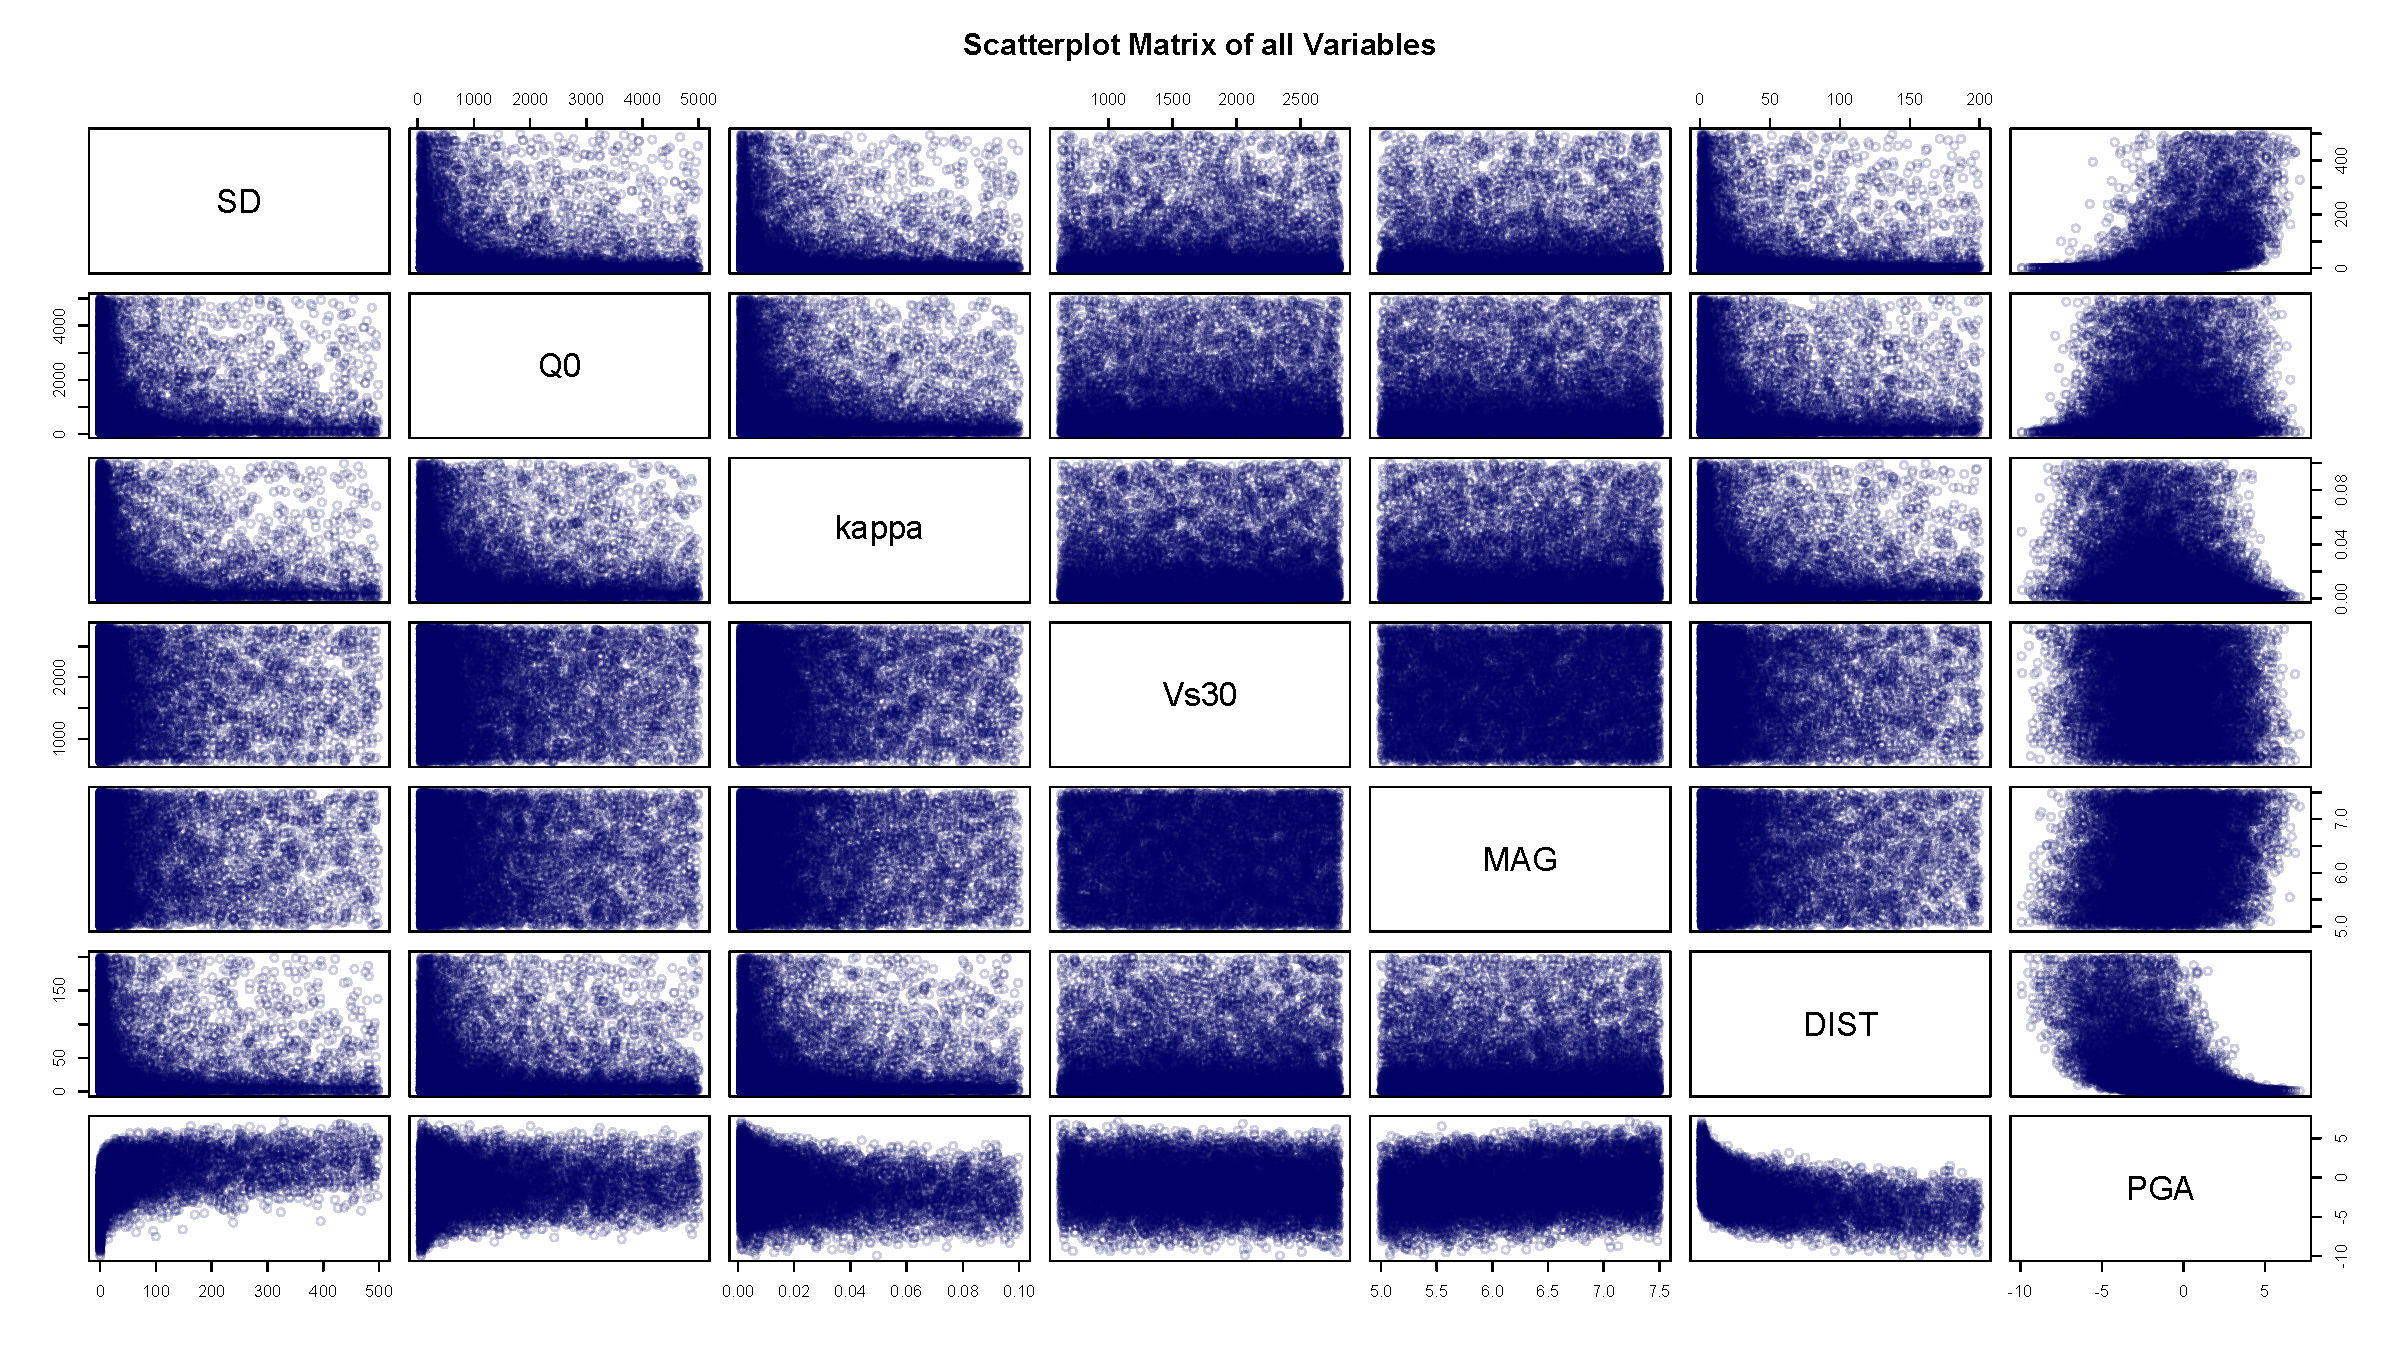
\includegraphics[scale=0.5]{Figures/allvsall.png}
		\rule{35em}{0.5pt}
	\caption[Scatterplot of all the variables]{Scatterplot of all the variables}
\end{figure}

\addtocontents{toc}{\vspace{2em}} % Add a gap in the Contents, for aesthetics

\backmatter

%----------------------------------------------------------------------------------------
%	BIBLIOGRAPHY
%----------------------------------------------------------------------------------------

\label{References}

\lhead{\emph{References}} % Change the page header to say "Bibliography"

\bibliographystyle{apa} % Use the "unsrtnat" BibTeX style for formatting the Bibliography

\bibliography{References} % The references (bibliography) information are stored in the file named "Bibliography.bib"

\end{document}  